\section{NFV Infrastructure}

\begin{flushleft}	
The NFV Infrastructure provides the necessary foundation for realizing all the pillars including MEC and NFV. The infrastructure mainly provides functions to automatically deploy and manage virtualized resources. Several requirements for NFV and MEC overlap and due to the similarities, a combined architecture for NFV and MEC was proposed in [2]. The idea is to use a common Infrastructure platform to run Virtual Application Functions (VAFs) and Virtual Network Functions (VNFs). The corresponding orchestration modules named as AFVO and NFVO. This common platform allows for reduced design issues and massive reuse of components thereby saving in CapeX and OpeX costs.
\end{flushleft}

\section{NFV Workloads}

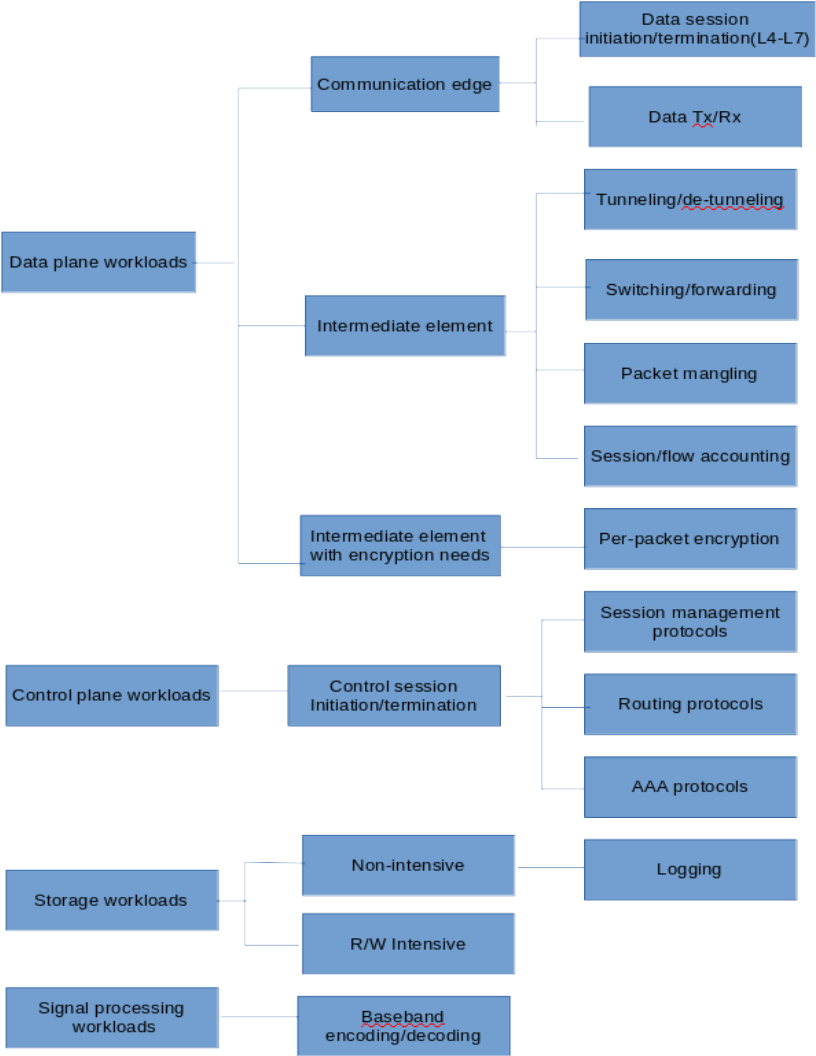
\includegraphics[width=0.9\textwidth]{workload_classification}
